\chapter{Hasil dan Analisis}

\section{Hasil Pemodelan Termal Satelit LAPAN-A3}

Gambar \ref{fig:node119} sampai dengan \ref{fig:node720} menunjukkan perbandingan suhu \textit{node-node} satelit
hasil prediksi model termal dengan data telemetri LAPAN-A3 aktual untuk periode observasi 19 sampai dengan 20 Mei 2018.

\begin{figure}[H]
\setlength\belowcaptionskip{-0.7\baselineskip}
\begin{center}
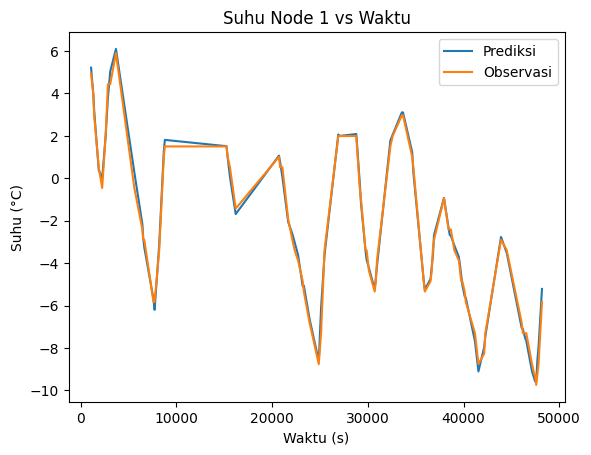
\includegraphics[width=0.6\textwidth]{fig/node1_temp_2018-05-19.png}
	\caption{Grafik suhu \textit{node} 1 vs waktu 19 Mei 2018}
\label{fig:node119}
\end{center}
\end{figure}

\begin{figure}[H]
\setlength\belowcaptionskip{-0.7\baselineskip}
\begin{center}
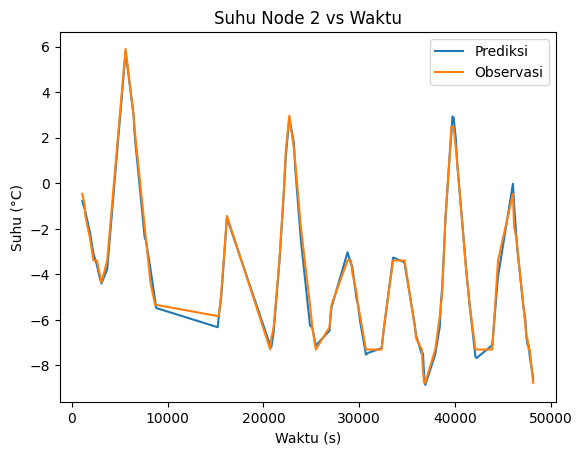
\includegraphics[width=0.6\textwidth]{fig/node2_temp_2018-05-19.png}
	\caption{Grafik suhu \textit{node} 2 vs waktu 19 Mei 2018}
\label{fig:node219}
\end{center}
\end{figure}

\begin{figure}[H]
\setlength\belowcaptionskip{-0.7\baselineskip}
\begin{center}
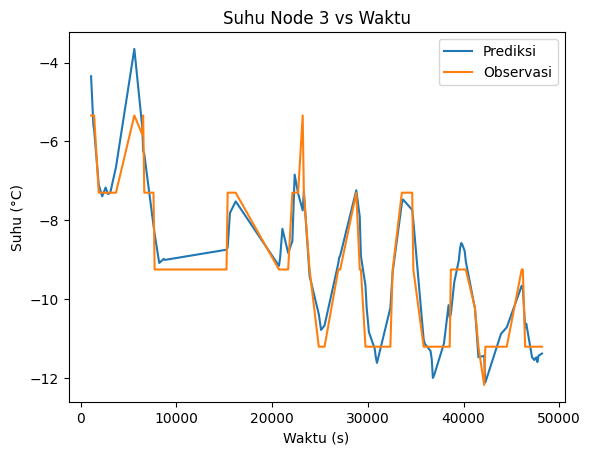
\includegraphics[width=0.6\textwidth]{fig/node3_temp_2018-05-19.png}
	\caption{Grafik suhu \textit{node} 3 vs waktu 19 Mei 2018}
\label{fig:node319}
\end{center}
\end{figure}

\begin{figure}[H]
\setlength\belowcaptionskip{-0.7\baselineskip}
\begin{center}
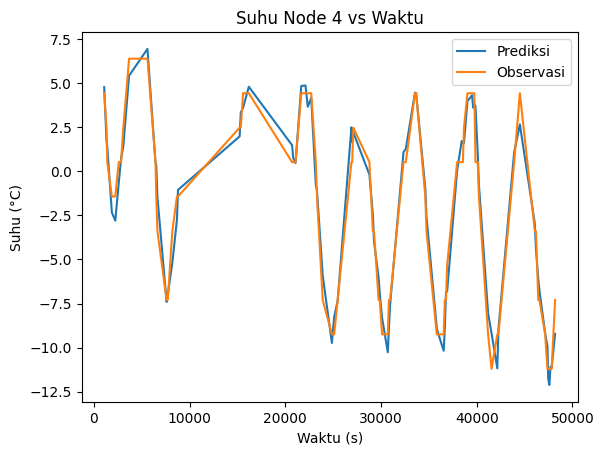
\includegraphics[width=0.6\textwidth]{fig/node4_temp_2018-05-19.png}
	\caption{Grafik suhu \textit{node} 4 vs waktu 19 Mei 2018}
\label{fig:node419}
\end{center}
\end{figure}

\begin{figure}[H]
\setlength\belowcaptionskip{-0.7\baselineskip}
\begin{center}
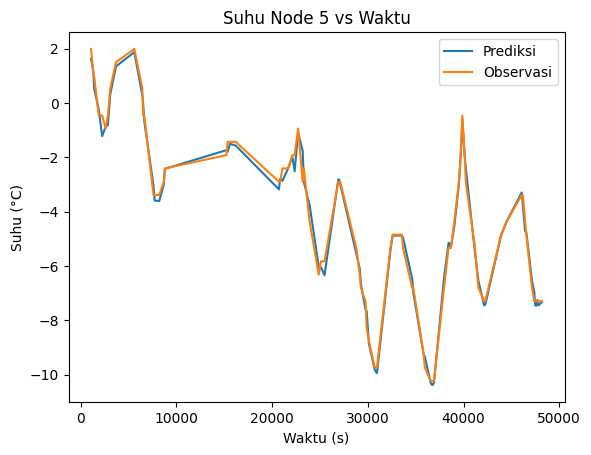
\includegraphics[width=0.6\textwidth]{fig/node5_temp_2018-05-19.png}
	\caption{Grafik suhu \textit{node} 5 vs waktu 19 Mei 2018}
\label{fig:node519}
\end{center}
\end{figure}

\begin{figure}[H]
\setlength\belowcaptionskip{-0.7\baselineskip}
\begin{center}
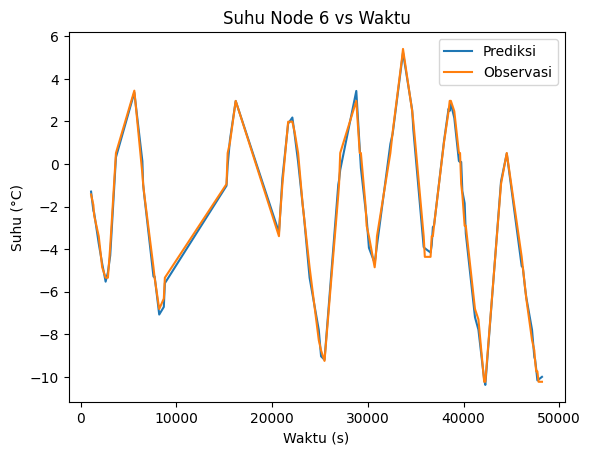
\includegraphics[width=0.6\textwidth]{fig/node6_temp_2018-05-19.png}
	\caption{Grafik suhu \textit{node} 6 vs waktu 19 Mei 2018}
\label{fig:node619}
\end{center}
\end{figure}

\begin{figure}[H]
\setlength\belowcaptionskip{-0.7\baselineskip}
\begin{center}
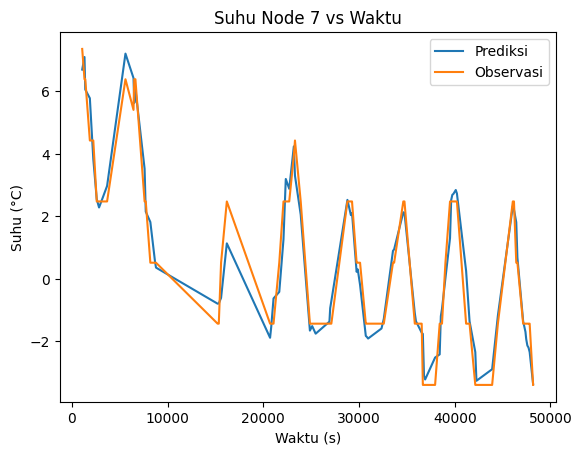
\includegraphics[width=0.6\textwidth]{fig/node7_temp_2018-05-19.png}
\caption{Grafik suhu \textit{node} 7 vs waktu 19 Mei 2018}
\label{fig:node719}
\end{center}
\end{figure}

\begin{figure}[H]
\setlength\belowcaptionskip{-0.7\baselineskip}
\begin{center}
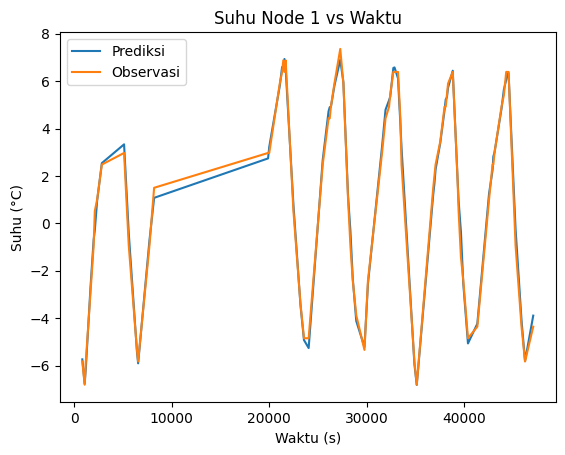
\includegraphics[width=0.6\textwidth]{fig/node1_temp_2018-05-20.png}
\caption{Grafik suhu \textit{node} 1 vs waktu 20 Mei 2018}
\label{fig:node120}
\end{center}
\end{figure}

\begin{figure}[H]
\setlength\belowcaptionskip{-0.7\baselineskip}
\begin{center}
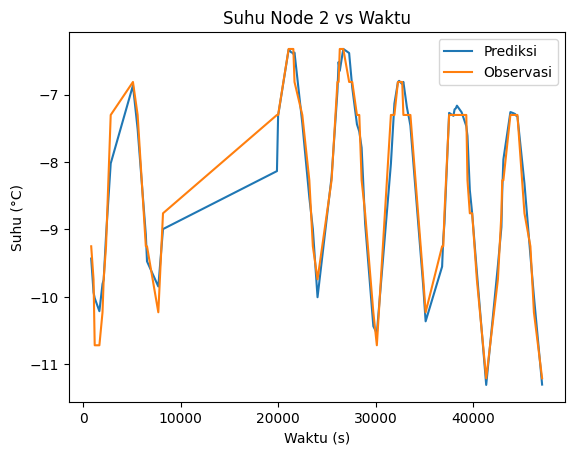
\includegraphics[width=0.6\textwidth]{fig/node2_temp_2018-05-20.png}
\caption{Grafik suhu \textit{node} 2 vs waktu 20 Mei 2018}
\label{fig:node220}
\end{center}
\end{figure}

\begin{figure}[H]
\setlength\belowcaptionskip{-0.7\baselineskip}
\begin{center}
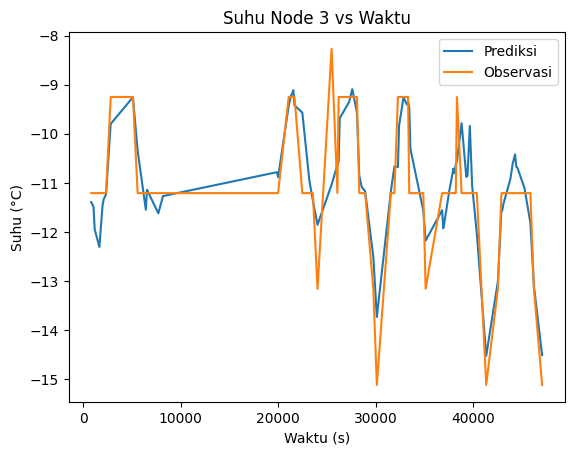
\includegraphics[width=0.6\textwidth]{fig/node3_temp_2018-05-20.png}
\caption{Grafik suhu \textit{node} 3 vs waktu 20 Mei 2018}
\label{fig:node320}
\end{center}
\end{figure}

\begin{figure}[H]
\setlength\belowcaptionskip{-0.7\baselineskip}
\begin{center}
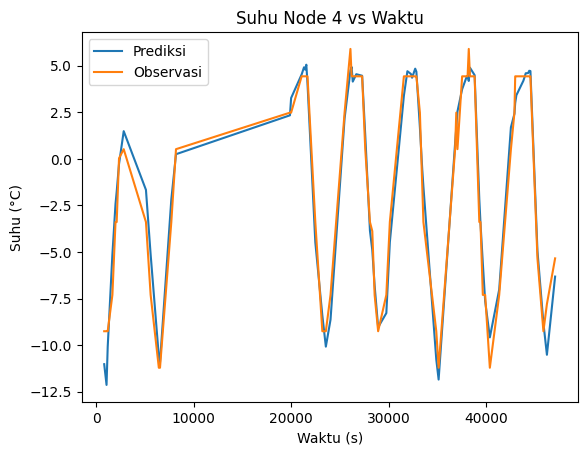
\includegraphics[width=0.6\textwidth]{fig/node4_temp_2018-05-20.png}
\caption{Grafik suhu \textit{node} 4 vs waktu 20 Mei 2018}
\label{fig:node420}
\end{center}
\end{figure}

\begin{figure}[H]
\setlength\belowcaptionskip{-0.7\baselineskip}
\begin{center}
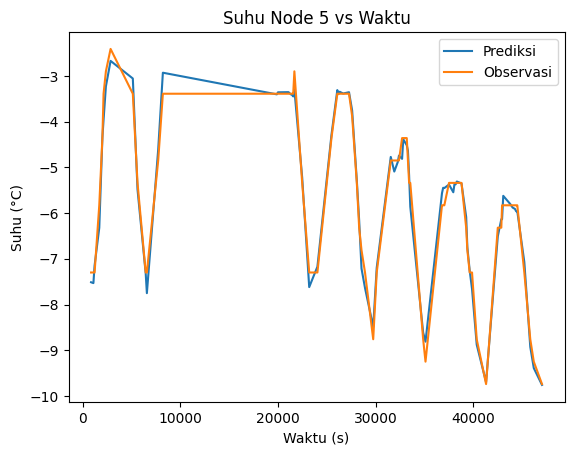
\includegraphics[width=0.6\textwidth]{fig/node5_temp_2018-05-20.png}
\caption{Grafik suhu \textit{node} 5 vs waktu 20 Mei 2018}
\label{fig:node520}
\end{center}
\end{figure}

\begin{figure}[H]
\setlength\belowcaptionskip{-0.7\baselineskip}
\begin{center}
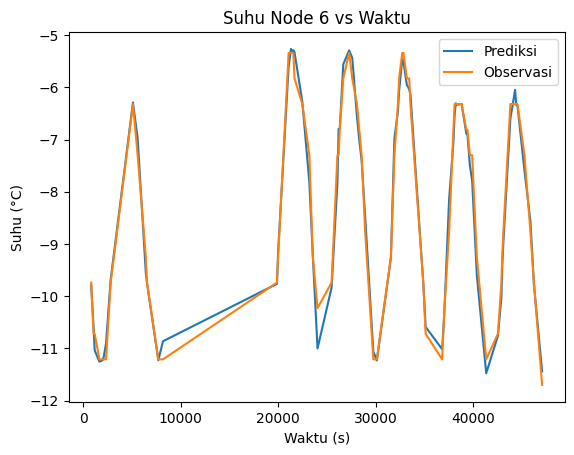
\includegraphics[width=0.6\textwidth]{fig/node6_temp_2018-05-20.png}
\caption{Grafik suhu \textit{node} 6 vs waktu 20 Mei 2018}
\label{fig:node620}
\end{center}
\end{figure}

\begin{figure}[H]
\setlength\belowcaptionskip{-0.7\baselineskip}
\begin{center}
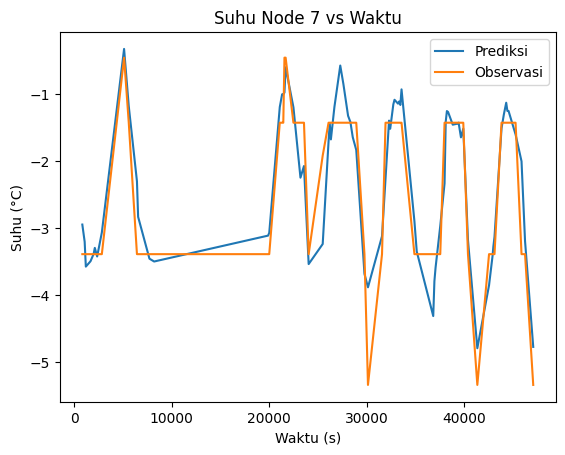
\includegraphics[width=0.6\textwidth]{fig/node7_temp_2018-05-20.png}
\caption{Grafik suhu \textit{node} 7 vs waktu 20 Mei 2018}
\label{fig:node720}
\end{center}
\end{figure}

Dapat dilihat bahwa model termal LAPAN-A3 dapat memprediksi kebanyakan tren
perubahan suhu \textit{node-node} satelit selama periode observasi dengan akurasi yang
cukup dekat dengan suhu observasi. Meskipun prediksi model termal mengalami
\textit{overshoot} dan \textit{undershoot}, model termal secara umum dapat
memprediksi apakah suhu \textit{node-node} satelit akan naik, turun, atau tetap sama
pada setiap selang waktu.

Meski demikian, node 3 dan 7 menghasilkan prediksi suhu
dengan tren yang cukup kontras dengan data suhu observasi. Perbedaan tren
prediksi suhu untuk kedua node terlihat paling jelas pada Gambar \ref{fig:node320}
dan \ref{fig:node720} yang memuat plot suhu \textit{node} 3 dan 7 terhadap waktu untuk
periode observasi 20 Mei 2018. Dari kedua grafik tersebut, dapat dilihat bahwa
model termal memprediksi perubahan suhu \textit{node} meski data telemetri suhu node
konstan seperti yang terjadi pada rentang waktu 10000 sampai dengan 20000
sekon.

Agar dapat dinilai secara kuantitatif, performa model termal dalam memprediksi
tren perubahan suhu \textit{node-node} satelit dapat dilihat dari hasil perhitungan skor koefisien determinasi $R^2$ prediksi suhu \textit{node-node} satelit pada Gambar \ref{fig:r219} dan
\ref{fig:r220}. Model termal LAPAN-A3 dapat menjelaskan mayoritas varians suhu
\textit{node} sehingga menghasilkan skor $R^2$ lebih dari 0.5 untuk semua \textit{node}. Lebih
lanjut, 6 dari 7 \textit{node} untuk periode 19 Mei 2018 dan 5 dari 7 \textit{node} untuk periode
20 Mei 2018 memiliki skor $R^2$ lebih besar dari 0.9. Ini berarti lebih dari 90\%
varians dalam data suhu observasi dapat dijelaskan oleh prediksi model. Dapat
dilihat juga bahwa \textit{node} 3 memiliki skor $R^2$ paling rendah dari ketujuh \textit{node} pada
kedua periode observasi dan disusul oleh \textit{node} 7.

\begin{figure}[H]
\setlength\belowcaptionskip{-0.7\baselineskip}
\begin{center}
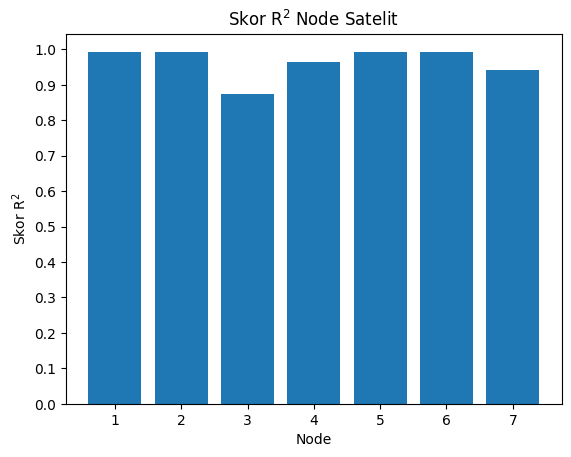
\includegraphics[width=0.6\textwidth]{fig/r2_2018-05-19.png}
\caption{Plot skor $R^2$ model 19 Mei 2018}
\label{fig:r219}
\end{center}
\end{figure}

\begin{figure}[H]
\setlength\belowcaptionskip{-0.7\baselineskip}
\begin{center}
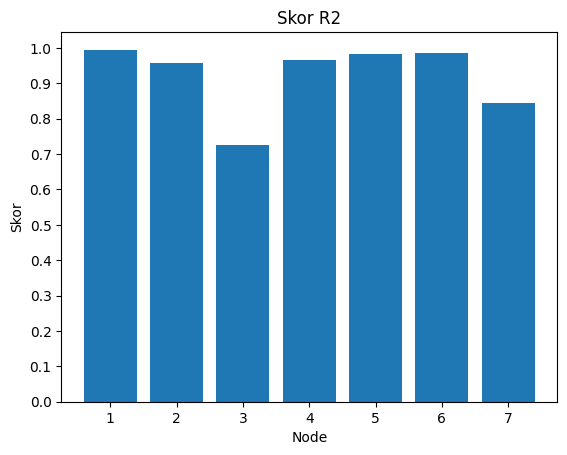
\includegraphics[width=0.6\textwidth]{fig/r2_2018-05-20.png}
\caption{Plot skor $R^2$ model 20 Mei 2018}
\label{fig:r220}
\end{center}
\end{figure}

Selanjutnya, keakuratan model termal dalam memprediksi suhu \textit{node} satelit pada
periode observasi dapat dilihat dari nilai \textit{root mean square error} (RMSE)
model yang mengukur seberapa jauh nilai suhu hasil prediksi model dengan nilai
suhu hasil observasi data telemetri. Gambar \ref{fig:rmse19} dan
\ref{fig:rmse20} memuat plot RMSE model termal. 

\begin{figure}[H]
\setlength\belowcaptionskip{-0.7\baselineskip}
\begin{center}
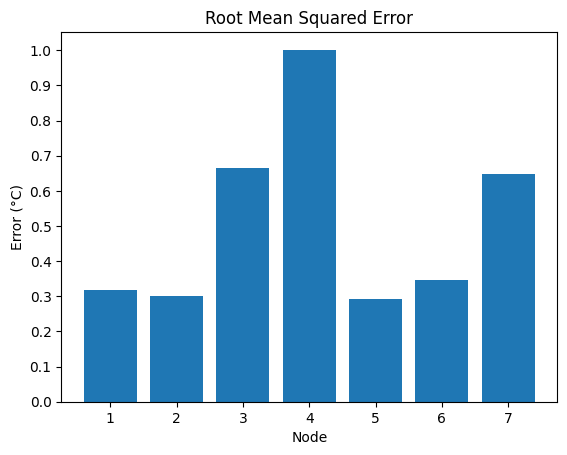
\includegraphics[width=0.6\textwidth]{fig/rmse_2018-05-19.png}
\caption{Plot nilai RMSE model 19 Mei 2018}
\label{fig:rmse19}
\end{center}
\end{figure}

\begin{figure}[H]
\setlength\belowcaptionskip{-0.7\baselineskip}
\begin{center}
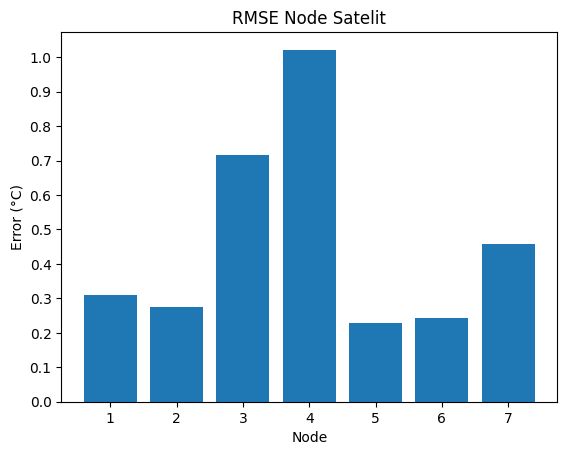
\includegraphics[width=0.6\textwidth]{fig/rmse_2018-05-20.png}
\caption{Plot nilai RMSE model 20 Mei 2018}
\label{fig:rmse20}
\end{center}
\end{figure}

Dapat dilihat bahwa plot RMSE model termal menunjukkan hasil yang agak berbeda
dari plot skor $R^2$ model termal pada Gambar \ref{fig:r219} dan \ref{fig:r220}
sebelumnya. Nilai RMSE paling besar untuk kedua periode observasi sama-sama
diperoleh dari \textit{node} 4 disusul oleh \textit{node} 3 dan kemudian \textit{node} 7. \textit{Node} 4 konsisten
memiliki nilai RMSE lebih besar sedikit dari 1 \degree C untuk kedua periode
observasi. \textit{Node} 3 juga konsisten memiliki nilai RMSE lebih besar dari 0.6
\degree C untuk kedua periode observasi sedangkan \textit{node} 7 sempat menyentuh nilai
di bawah 0.5 \degree C pada periode observasi 20 Mei 2018.

\section{Analisis}

Hasil pemodelan termal satelit LAPAN-A3 dari bagian sebelumnya menunjukkan
bahwa model termal yang dikembangkan sudah dapat memodelkan karakteristik
termal satelit LAPAN-A3 secara umum. Akan tetapi, akurasi model termal satelit
dalam memodelkan karakteristik termal \textit{node} 3, 4, dan 7 dapat dikatakan lebih
rendah dibandingkan dengan 4 \textit{node} lainnya dan masih perlu ditingkatkan. Node 3
dan 7 konsisten memiliki skor $R^2$ lebih rendah dibandingkan \textit{node}-\textit{node} lainnya
sedangkan \textit{node} 4 memiliki nilai RMSE paling besar untuk kedua periode
observasi.

Dalam menganalisis hasil pemodelan termal, perlu diingat bahwa metrik performa
model yang dihitung hanya berlaku untuk iterasi dan konfigurasi parameter model
\textit{machine learning} saat ini. Sebagai contoh, perubahan parameter
\textit{seed number} yang digunakan akan mengubah dataset latihan dan ujian
model. Hal ini akan mengubah hasil prediksi model dan tentunya juga akan mengubah
akurasi prediksi model termal. 

Selanjutnya, seperti yang disebutkan pada bab Tinjauan Pustaka, parameter RMSE
bergantung pada skala pemodelan dan dataset yang digunakan. Karena itu,
perbedaan nilai maksimum dan minimum RMSE baru dapat disimpulkan setelah ada
perbandingan dengan model termal di masa depan. Dengan kata lain, belum dapat
disimpulkan apakah nilai RMSE model termal saat ini dapat dikategorikan rendah
atau tinggi.

Terlepas dari ketidakpastian dan ketidakakuratan bawaan dari metode numerik dan
\textit{machine learning} yang digunakan pada karya tulis ini, dapat diduga
bahwa model satelit LAPAN-A3 yang digunakan belum dapat mewakili seluruh
karakteristik termal satelit. Dengan menganalisis sumber ketidakakuratan model
yang potensial, model termal satelit dapat dikembangkan lebih lanjut pada
iterasi berikutnya. Harapannya, iterasi model termal satelit berikutnya dapat
menunjukkan performa yang jauh lebih akurat lagi.

Pertama, satelit LAPAN-A3 didekati dengan model 7 \textit{node} diskrit yang
mewakili 6 sisi satelit serta 1 plat tengah satelit. \textit{Node} digunakan sebagai
satuan titik analisis terkecil sehingga bagian satelit yang diwakili \textit{node}
dianggap memiliki suhu yang sama. Parameter kapasitas termal yang digunakan
pada persamaan-persamaan termal di karya tulis ini pun adalah nilai kapasitas
termal rata-rata \textit{node}. 

\textit{Node} satelit yang terdiri dari material dan komponen yang berbeda dapat
menghasilkan rentang kapasitas termal \textit{node} yang besar juga. Rentang kapasitas
termal yang besar berarti rentang perubahan suhu antar material dalam \textit{node} yang
besar juga. Akibatnya, bacaan sensor suhu bisa saja berbeda jauh dengan suhu
komponen masing-masing sebenarnya.

Dalam konteks LAPAN-A3, \textit{node} 3 terletak di sumbu Y+ satelit yang memuat adaptor
roket dan \textit{separation ring} sedangkan \textit{node} 7 terletak di plat tengah
satelit yang menyimpan banyak komponen seperti komputer satelit dan sub-sistem
lainnya. Dengan begitu, karakteristik termal material pada kedua \textit{node} mungkin
tidak dapat terwakili seluruhnya dalam model satelit 7 \textit{node}. Agar karakteristik
termal dapat dimodelkan lebih akurat, jumlah \textit{node} yang digunakan dalam
pemodelan dapat ditambah.

Kemudian, satelit LAPAN-A3 juga diasumsikan berbentuk balok sehingga
perhitungan \textit{view factor} dari \textit{node} ke Bumi disederhanakan
menjadi plat persegi panjang ke Bumi. Pada kenyataannya, satelit memiliki
komponen yang tidak berbentuk persegi panjang seperti antena dan kamera.
Penambahan jumlah \textit{node} untuk memastikan komponen-komponen tersebut
terwakili tentunya juga akan menambah akurasi dari model termal satelit. Selain
itu, tidak tertutup juga penggunaan metode numerik lain seperti metode elemen
hingga untuk menghitung nilai \textit{view factor} secara terpisah agar data
\textit{view factor} yang digunakan untuk melatih model dapat lebih mendekati
nilai \textit{view factor node} satelit yang sebenarnya.

Lalu, dari Persamaan \ref{eq:lineq} dapat dilihat juga bahwa perubahan suhu
suatu \textit{node} dipengaruhi perubahan suhu \textit{node} lain akibat adanya
perpindahan panas lewat konduksi dan radiasi antar \textit{node}. Merujuk
aplikasi lain dari \textit{machine learning} pada pemodelan termal satelit,
analisis inferensi dapat dilakukan untuk menentukan variabel-variabel dominan
dalam Persamaan \ref{eq:lineq} yang mungkin menyumbang \textit{error} paling
besar. Jika hasil inferensi menunjukkan bahwa perubahan suhu \textit{node} 4
didominasi oleh pengaruh perubahan suhu \textit{node} 3 dan 7, penjelasan
sebelumnya dapat turut menjawab hasil nilai RMSE \textit{node} 4. Sebaliknya,
hasil analisis tersebut dapat digunakan untuk melihat akurasi suku termal mana
yang perlu ditingkatkan agar perbedaan antara nilai hasil prediksi model dengan
data observasi dapat dikurangi.

Analisis inferensi untuk mengetahui kontribusi tiap variabel dalam Persamaan
\ref{eq:lineq} membutuhkan modifikasi metode \textit{machine learning} yang
digunakan. Dapat dilihat dari persamaan tersebut bahwa variabel suhu
\textit{node} berkorelasi erat dengan variabel suhu \textit{node} pangkat 4.
Jika salah satu variabel diketahui, variabel lainnya dapat dihitung juga.
Fenomena adanya korelasi tinggi antar variabel independen tersebut dinamakan
kolinearitas. 

Meski kolinearitas tidak berdampak banyak pada akurasi prediksi model regresi
linear, hal ini harus diperhitungkan dalam analisis inferensi
\cite{lieberman2014}\cite{mundfrom2018}. Kolinearitas sendiri dapat diatasi
dengan menyeleksi variabel independen sehingga tidak ada kolinearitas pada
variabel yang tersisa atau menggunakan metode \textit{machine learning} lain
yang tidak terpengaruh kolinearitas.

Analisis inferensi persamaan termal tidak dilakukan pada karya tulis ini karena
model termal yang dikembangkan pada karya tulis ini memiliki tujuan utama
berupa prediksi suhu satelit. Meski demikian, topik tersebut dapat menjadi
bahan pengembangan model termal selanjutnya atau topik penelitian lebih lanjut
di masa depan. Dengan begitu, model termal satelit LAPAN-A3 dapat dikembangkan
lebih baik lagi.
